\section{Хэш-функция «Стрибог»}\label{section-stribog}\index{хэш-функция!«Стрибог»|(}
\selectlanguage{russian}

С 1 января 2013 года в России введён в действие новый стандарт на криптографическую хэш-функцию ГОСТ Р 34.11-2012~\cite{GOST-R:34.11-2012}. Неофициально новый алгоритм получил название <<Стрибог>>. При разработке хэш-функции авторы основывались на нескольких требованиях:

\begin{itemize}
	\item не должна быть уязвима к известным атакам;
	\item должна использовать хорошо изученные конструкции и преобразования;
	\item не должно быть лишних преобразований, каждое преобразование должно гарантировать выполнение определённых криптографических свойств;
	\item при наличии нескольких вариантов реализации требуемого свойства -- наиболее простой для анализа и реализации;
	\item максимальная производительность \emph{программной} реализации.
\end{itemize}

В соответствии с данными требованиями алгоритм новой хэш-функции основывается на хорошо изученных конструкциях Меркла~---~Дамгарда\index{структура!Меркла~---~Дамгарда}~\cite{Merkle:1979, Merkle:1990, Damgard:1990} и Миагучи~---~Пренеля\index{структура!Миагучи~---~Пренеля}~\cite{Espen:Mieghem:1989, Miyaguchi:Ohta:Iwata:1990:03, Miyaguchi:Ohta:Iwata:1990:11}, во внешней своей структуре практически полностью повторяя режим HAIFA\index{HAIFA} (\langen{HAsh Iterative FrAmework},~\cite{Biham:Dunkelman:2007}), использовавшийся в хэш-функциях SHAvite-3\index{хэш-функция!SHAvite-3} и BLAKE\index{хэш-функция!BLAKE}.

\begin{figure}[htb]
	\centering
	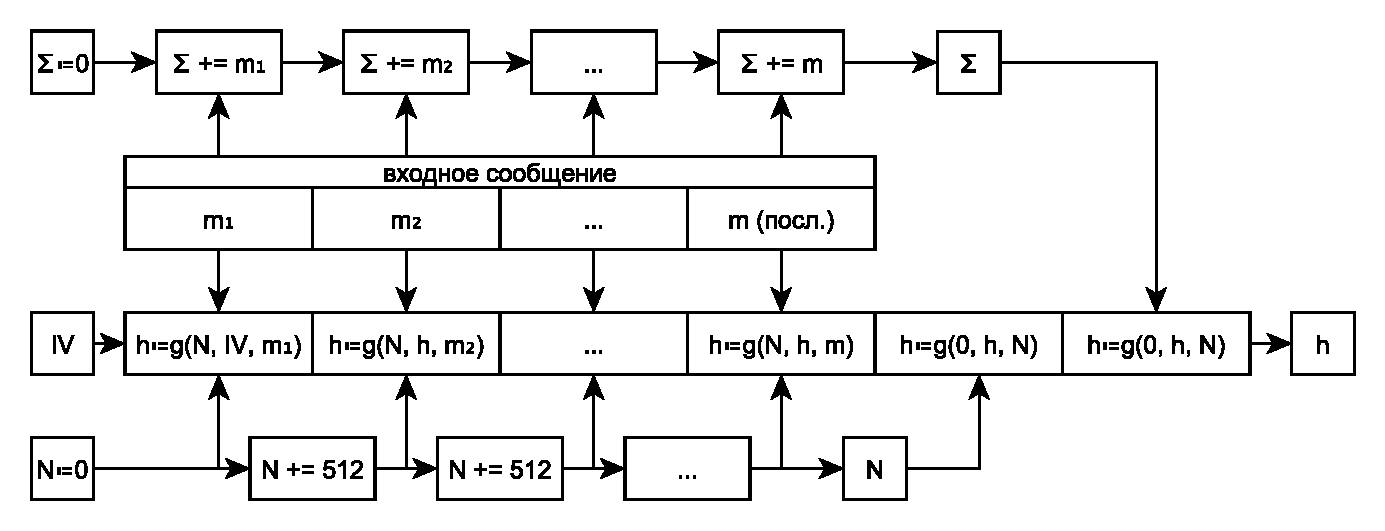
\includegraphics[width=0.95\textwidth]{pic/stribog-md}
  \caption{Использование структуры Меркла~---~Дамгарда в хэш-функции <<Стрибог>>}
  \label{fig:stribog-md}
\end{figure}

Как показано на рис.~\ref{fig:stribog-md}, входное сообщение разбивается на блоки по 512 бит (64 байта). Последний блок \emph{слева} дополняется последовательностью из нулей и  одной единицы до 512 бит (длина дополнения не учитывается в дальнейшем, когда длина сообщения используется как аргумент функций). Для каждой части сообщения вычисляется значение функции $g_N(h, m)$, которая в качестве аргумента использует текущий номер блока (умноженный на 512), результат вычисления для предыдущего блока и очередной блок сообщения. Также есть два завершающих преобразования. Первое вместо блока сообщения использует количество обработанных бит N (то есть длину сообщения), а второе -- арифметическую сумму значений всех блоков сообщения. В предположении, что функция $g_N(h, m)$ является надёжной для создания криптографически стойких хэш-функций, известно, что конструкция Меркла~---~Дамгарда позволяет получить хэш-функцию со следующими параметрами:

\begin{itemize}
	\item сложность построения прообраза: $2^n$ операций;
	\item сложность построения второго прообраза: $2^n / \left|M\right|$ операций;
	\item сложность построения коллизии: $2^{n/2}$ операций;
	\item сложность удлинения прообраза: $2^n$ операций.
\end{itemize}

Все параметры совпадают с аналогичными для идеальной хэш-функции, кроме сложности построения второго прообраза, который равен $2^n$ для идеального алгоритма.

В качестве функции $g_N(h, m)$ используется конструкция Миагучи~---~Пренеля\index{структура!Миагучи~---~Пренеля} (см. рис.~\ref{fig:stribog-mp}), которая является стойкой ко всем атакам, известным для схем однонаправленных хэш-функций на базе симметричных алгоритмов, в том числе к атаке с <<фиксированной точкой>>~\cite[стр. 502]{Schneier:2002}. \emph{Фиксированной точкой}\index{точка!фиксированная} называется пара чисел $(h, m)$, для которой у заданной функции $g$ выполняется $g(h, m) = h$.

\begin{figure}[htb]
	\centering
	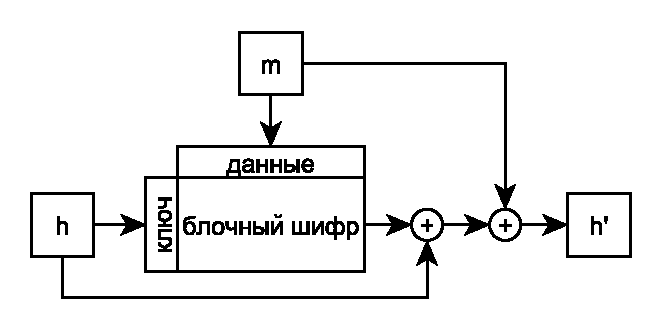
\includegraphics[width=0.66\textwidth]{pic/stribog-mp}
  \caption{Использование структуры Миагучи~---~Пренеля в хэш-функции <<Стрибог>>}
  \label{fig:stribog-mp}
\end{figure}

\index{шифр!XSPL|(}В качестве блочного шифра используется новый XSPL-шифр, изображённый на рис.~\ref{fig:stribog-xspl}, отдельные элементы и идеи которого позже войдут в новый стандарт <<Кузнечик>>\index{шифр!<<Кузнечик>>} (см. раздел~\ref{section-grig}). Шифр является примером шифра на основе SP-сети\index{SP-сеть} (сети замен и перестановок), каждый раунд которого является набором обратимых преобразований над входным блоком.

\begin{figure}[htb]
	\centering
	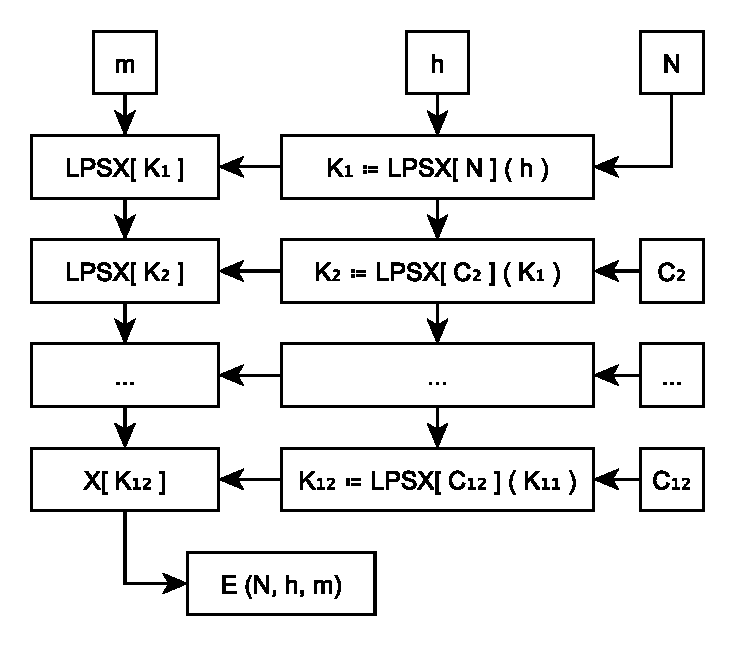
\includegraphics[width=0.75\textwidth]{pic/stribog-xspl}
  \caption{XSPL-шифр в хэш-функции <<Стрибог>>}
  \label{fig:stribog-xspl}
\end{figure}

Каждый раунд XSPL-шифра, кроме последнего, состоит из следующих обратимых преобразований:
\begin{itemize}
	\item $X\left[C\right]$ -- побитовое сложение по модулю 2 с дополнительным аргументом $C$;
	\item $S$ -- нелинейная обратимая замена байтов;
	\item $P$ -- перестановка байтов внутри блока данных (транспонирование матрицы размером $8 \times 8$ из ячеек по одному байту каждая);
	\item $L$ -- обратимое линейное преобразование (умножение векторов на фиксированную матрицу).
\end{itemize}

Особенностью предложенного шифра является полная аналогия между алгоритмом развёртывания ключа и алгоритмом, собственно, преобразования открытого текста. В качестве <<раундовых ключей>> для алгоритма развёртывания ключа на первом раунде используется общее число уже обработанных бит хэш-функцией N, а на остальных раундах -- 512-битные константы, заданные в стандарте.\index{шифр!XSPL|)}

Новый алгоритм, согласно отдельным исследованиям, до полутора раз быстрее предыдущего стандарта ГОСТ Р 34.11-94\index{хэш-функция!ГОСТ Р 34.11-94}, используя 27 тактов на один байт входного сообщения (94~МБ/с), против 40 для старого стандарта (64~МБ/с)\footnote{Реализации тестировались на процессоре Intel Core i7-920 CPU @ 2.67~GHz и видеокарте NVIDIA GTX 580. См.~\cite{Lebedev:2013}.}.

В 2014 году группа исследователей (\cite{Guo:Jean:Leurent:Peyrin:Wang:2014}) обнаружила недостаток в реализации конструкции HAIFA в хэш-функции <<Стрибог>>, который ведёт к уменьшению сложности атаки по поиску второго прообраза до $n \times 2^{n/2}$, то есть до $2^{266}$. Авторы работы получили первую премию в размере пятьсот тысяч рублей на конкурсе по исследованию хэш-функции «Стрибог», проводившемся Российским Техническим комитетом по стандартизации «Криптографическая защита информации» (ТК~26) при участии Академии криптографии Российской Федерации и при организационной и финансовой поддержке ОАО «ИнфоТеКС».

\index{хэш-функция!«Стрибог»|)}
